\documentclass[a4paper,11pt]{article}

% Márgenes ajustados (poco generosos)
\usepackage[margin=1.5cm]{geometry}

% Soporte para idioma y codificación
\usepackage[utf8]{inputenc}
\usepackage[catalan,spanish]{babel}

% Paquetes para la tabla de la cabecera e imágenes
\usepackage{tabularx}
\usepackage{array}
\usepackage{graphicx} % Necesario para incluir las imágenes

% Paquetes para numeración de páginas estilo X/Y
\usepackage{fancyhdr}
\usepackage{lastpage}

\usepackage{multirow}
\usepackage[table]{xcolor}
\usepackage{titlesec}
\definecolor{grisclar}{gray}{0.85}

\renewcommand{\arraystretch}{1.4}
\setlength{\tabcolsep}{3pt}

% Configuración de cabeceras y pies de página
\pagestyle{fancy}
\fancyhf{} % Limpiar cabeceras y pies
\renewcommand{\headrulewidth}{0pt} % Sin línea en la cabecera
\cfoot{\thepage/\pageref{LastPage}} % Numeración en el centro del pie de página


%-----------------------------------------------------
%-----------------------------------------------------
% ---- Fixed column widths, computed ONCE from the true page width. ----
% (Using "0.34\linewidth" etc. directly *inside* the table cells would be wrong:
%  a p{} column locally redefines \linewidth to its own (already narrow) width,
%  so nested fractions would compound. Capturing plain lengths here avoids that.)
\newlength{\ca} \setlength{\ca}{0.080\textwidth} % logo Generalitat
\newlength{\cb} \setlength{\cb}{0.25\textwidth} % text block
\newlength{\cc} \setlength{\cc}{0.170\textwidth} % "Curs ..."
\newlength{\cd} \setlength{\cd}{0.21\textwidth} % DEPARTAMENT / TRIMESTRE / UNITAT
\newlength{\ce} \setlength{\ce}{0.085\textwidth} % "Grup:" / "NOTA:" label width
\newlength{\cf} \setlength{\cf}{0.130\textwidth} % logo Institut / value width

\newlength{\colA} \setlength{\colA}{\ca}\addtolength{\colA}{1.5cm} % label "Nom i cognoms:" / "Data:"
\newlength{\colB} \setlength{\colB}{\cc}\addtolength{\colB}{\cd} % value cell (wide, blank)
\newlength{\colC} \setlength{\colC}{\cd}\addtolength{\colC}{4.5cm} 
\newlength{\rowfullwidth} \setlength{\rowfullwidth}{\ca}
  \addtolength{\rowfullwidth}{\cb}\addtolength{\rowfullwidth}{\cc}
  \addtolength{\rowfullwidth}{\cd}\addtolength{\rowfullwidth}{\ce}\addtolength{\rowfullwidth}{\cf}
%-----------------------------------------------------
%-----------------------------------------------------

% =========================================================
% DEFINICIÓN DE VARIABLES PARA EL PREFACIO (CABECERA)
% =========================================================
\makeatletter
\newcommand{\departament}[1]{\def\@departament{#1}}
\newcommand{\trimestre}[1]{\def\@trimestre{#1}}
\newcommand{\unitat}[1]{\def\@unitat{#1}}
\newcommand{\instruccions}[1]{\def\@instruccions{#1}}

% Valores por defecto
\departament{Ciències experimentals}
\trimestre{1er Trimestre}
\unitat{}
\instruccions{}

% Comando para renderizar la tabla en la primera página
\newcommand{\crearcabecera}{
    \noindent
    \begin{tabular}{|p{\ca}p{\cb}|p{\cc}p{\cd}p{\ce}p{\cf}|}
\hline

% ---------- Header block (3 rows) ----------
\multirow{3}{*}{
\includegraphics[width=\ca]{senyal_bn.png}}
 & \multirow{3}{\cb}{Generalitat de Catalunya\\ Departament d'educaci\'o i\\ Formaci\'o professional}
 & \multicolumn{3}{p{\colB}}{\textbf{\@departament}}
 & \multirow{3}{*}{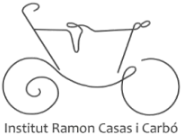
\includegraphics[width=\cf]{RCC.png}} \\
 & & \multicolumn{3}{p{\colB}}{\@trimestre} & \\
 & & \multicolumn{3}{p{\colC}}{\textit{\@unitat}} & \\
\hline

% ---------- Nom i cognoms / Grup ----------
\multicolumn{2}{|p{\colA}}{\cellcolor{grisclar}Nom i cognoms:}
 & \multicolumn{2}{p{\colB}|}{}
 & \cellcolor{grisclar}Grup:
 & \\
\hline

% ---------- Data / Nota ----------
\multicolumn{2}{|p{\colA}}{\cellcolor{grisclar}Data:}
 & \multicolumn{2}{p{\colB}|}{}
 & \cellcolor{grisclar}\textbf{Nota:}
 & \\
\hline

% ---------- Instruccions ----------
\multicolumn{6}{|p{\rowfullwidth}|}{%

  \hspace{0.5em}\textbf{Instruccions de la prova:} \vspace{0.4em} \newline 
    \hspace*{1.5em}\begin{minipage}{0.9\linewidth}
        \@instruccions
        \vspace{0.4em}
    \end{minipage}
} \\
\hline

\end{tabular}
    
    \vspace{1em}
}
\makeatother

% =========================================================
% DEFINICIÓN DEL ENTORNO DE EJERCICIOS
% =========================================================
\newcounter{numexercici}
\newenvironment{exercici}[1][]{%
    \refstepcounter{numexercici}%
    \vspace{1em}\noindent\textbf{Exercici \thenumexercici.} 
    % Si se proporciona el argumento de los puntos, lo imprime
    \ifx&#1&\else \textit{(#1 punts)}\fi
    \par\vspace{0.3em}\noindent\ignorespaces
}{%
    \par\vspace{0.5em}
}

% Configuració de títols d'exercicis
\titleformat{\section}{\large\bfseries}{Exercici \thesection.}{0.5em}{}



% =========================================================
% RELLENAR DATOS DEL EXAMEN AQUÍ (PREFACIO)
% =========================================================
\departament{Física 1er Batx 26-27}
\trimestre{1r Trimestre}
\unitat{Unitat 0. Repàs 1er batxillerat. Amb apunts.}
\instruccions{
    Es pot fer servir un formulari fet per tu, un foli amb informació per les dues cares. \\
    Totes les respostes s’han de raonar i justificar. Un resultat erroni amb un raonament correcte es valora. Una resposta correcta sense raonament ni justificació pot ser valorada amb un 0.\\
    Un o més errors d’unitats o no posar-les (resultats intermedis i finals) en un problema es penalitzen amb un 20\% del valor del exercici. \\
    Es permet l'ús de calculadora científica no programable.
}

\begin{document}

% 1. Insertamos la tabla de cabecera
\crearcabecera

% 2. Ejemplos de uso de los ejercicios

Un vagó de muntanya russa ($m = 7\times 10^{-29} M_\odot$) es mou a $v_0 = 25.2$ km/h quan passa a una alçada de $h_0 = 4.5\times 10^{10} $ nanòmetres del terra. El fregament amb l'aire i el carril és negligible\footnote{\textbf{Dades:} $1 M_\odot = 1.988 \times 10^{30}$ kg. $g = 9.8$ m/s$^2$.}.
\begin{figure}[h!]
    \centering
    \includegraphics[width=0.5\linewidth]{loop.png}
\end{figure}
\vspace{-0.5cm}
\section{(1.5 punts)}
Expressa tots els valors del enunciat en Sistema Internacional, fent servir factors de conversió.
\section{(1 punt)}
Calcula la velocitat amb que arribarà al terra (punt $A$) el vagó. Explica quins principis has fet servir.
\section{(2.5 punts)}
La muntanya russa té un loop circular de radi $R = 15$ metres. Calcula amb quina velocitat arribarà el vagó al punt més alt, i raona si tindrà prou velocitat per no caure. 
\section{(2 punts)}
Calcula el radi màxim que podria tenir el loop per tal de que el vagó no caiguès. 
\section{(2 punts)}
Després del loop (punt $B$), en un tram horitzontal a la mateixa alçada que el punt $A$, el primer vagò col·lisiona amb un altre vagó que es trova en repós i que té la meitat de massa. Després de la col·lisió queden enganxats i es mouen conjuntament. Calcula quin és modul de la velocitat final del conjunt. 
\section{(1 punt)}
Raona com canvia cada resultat si la massa dels vagons fos 10 vegades més elevada. 



\end{document}


\begin{tabularx}{\textwidth}{|>{\centering\arraybackslash}m{6cm}|X|>{\centering\arraybackslash}m{3cm}|}
        \hline
        % Columna 1: senyal_bn.png
        
\includegraphics[width=2.5cm,height=2cm,keepaspectratio]{senyal_bn.png} \mbox{Generalitat de Catalunya\\ Departament d'Educació i\\Formació professional }& 
        % Columna 2: Datos
        \textbf{Departament:} \@departament \newline
        \textbf{Trimestre:} \@trimestre \newline
        \textbf{Unitat:} \@unitat & 
        % Columna 3: im2.png
        \includegraphics[width=2.5cm,height=2cm,keepaspectratio]{im2.png} \\
        \hline
        % Fila 2: Instrucciones abarcando las 3 columnas
        % Minipage asegura que podamos usar saltos de línea (\\) sin romper la tabla
        \multicolumn{3}{|p{\dimexpr\textwidth-2\tabcolsep-2\arrayrulewidth}|}{
            \textbf{Instruccions de la prova:} \vspace{0.3em} \newline 
            \begin{minipage}{\linewidth}
                \@instruccions
                \vspace{0.2em}
            \end{minipage}
        } \\
        \hline
    \end{tabularx}